\documentclass[12pt]{article}
\usepackage[utf8]{inputenc}
\usepackage[T1]{fontenc}
\usepackage[spanish]{babel}
\usepackage{listings}
\usepackage{graphicx}
\usepackage{geometry}
\usepackage{enumitem}
\geometry{margin=2.5cm}

% Configuración de listings
\lstset{
    basicstyle=\ttfamily\small,
    breaklines=true,
    frame=single,
    showstringspaces=false,
    tabsize=2
}

\title{Actualización Automática de Salarios y Categorías}
\author{Aaron Rodrigo Ramos Reyes}
\date{\today}

\begin{document}

\maketitle

\section*{Planteamiento del problema}
Se deben crear dos tablas:
\begin{itemize}[leftmargin=*]
    \item \textbf{Empleados}: con nombre, puesto, fecha de ingreso y salario
    \item \textbf{Tabulador}: con nombre del puesto, días necesarios y salario correspondiente
\end{itemize}

Diagrama ER planteado como solución:
\begin{center}
    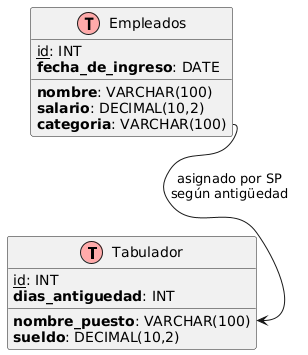
\includegraphics[width=0.7\textwidth]{DiagramaER.png}
\end{center}

\section*{Implementación en SQL}
\subsection*{Creación de la base de datos y tablas}
\begin{lstlisting}[language=SQL]
CREATE DATABASE EMPRESA;
USE EMPRESA;

CREATE TABLE Empleados (
    id INT AUTO_INCREMENT PRIMARY KEY,
    nombre VARCHAR(100),
    fecha_de_ingreso DATE,
    salario DECIMAL(10,2),
    categoria VARCHAR(100)
);

CREATE TABLE Tabulador (
    id INT AUTO_INCREMENT PRIMARY KEY,
    nombre_puesto VARCHAR(100),
    sueldo DECIMAL(10,2),
    dias_antiguedad INT
);
\end{lstlisting}

\subsection*{Datos iniciales para Tabulador}
\begin{lstlisting}[language=SQL]
INSERT INTO Tabulador (nombre_puesto, sueldo, dias_antiguedad) VALUES 
    ('Trainee', 1000.00, 1),
    ('Dev Junior', 5000.00, 12),
    ('Dev Senior', 10000.00, 20);
\end{lstlisting}

\subsection*{Empleados de prueba}
\begin{lstlisting}[language=SQL]
INSERT INTO Empleados (nombre, fecha_de_ingreso, salario, categoria) VALUES
    ('Ana Torres',       CURDATE() - INTERVAL 1 DAY,  0.00, 'Por definir'),
    ('Luis Gomez',       CURDATE() - INTERVAL 2 DAY,  0.00, 'Por definir'),
    ('Maria Lopez',      CURDATE() - INTERVAL 3 DAY,  0.00, 'Por definir'),
    ('Carlos Mendez',    CURDATE() - INTERVAL 5 DAY,  0.00, 'Por definir'),
    ('Julia Rios',       CURDATE() - INTERVAL 7 DAY,  0.00, 'Por definir'),
    ('Pedro Jimenez',    CURDATE() - INTERVAL 9 DAY,  0.00, 'Por definir'),
    ('Lucia Castro',     CURDATE() - INTERVAL 10 DAY, 0.00, 'Por definir'),
    ('Miguel Serrano',   CURDATE() - INTERVAL 12 DAY, 0.00, 'Por definir'),
    ('Elena Vargas',     CURDATE() - INTERVAL 15 DAY, 0.00, 'Por definir'),
    ('Jorge Pena',       CURDATE() - INTERVAL 18 DAY, 0.00, 'Por definir'),
    ('Valeria Cruz',     CURDATE() - INTERVAL 20 DAY, 0.00, 'Por definir'),
    ('Santiago Ruiz',    CURDATE() - INTERVAL 22 DAY, 0.00, 'Por definir'),
    ('Gabriela Mora',    CURDATE() - INTERVAL 25 DAY, 0.00, 'Por definir'),
    ('Hugo Castillo',    CURDATE() - INTERVAL 27 DAY, 0.00, 'Por definir'),
    ('Laura Fernandez',  CURDATE() - INTERVAL 30 DAY, 0.00, 'Por definir');
\end{lstlisting}

\subsection*{Stored Procedure para actualización}
\begin{lstlisting}[language=SQL]
DELIMITER $$

CREATE PROCEDURE ActualizarSalarioYCategoria()
BEGIN
    UPDATE Empleados e
    JOIN (
        SELECT 
            e.id,
            t.nombre_puesto,
            t.sueldo
        FROM Empleados e
        JOIN Tabulador t
            ON DATEDIFF(CURDATE(), e.fecha_de_ingreso) >= t.dias_antiguedad
        WHERE t.dias_antiguedad = (
            SELECT MAX(t2.dias_antiguedad)
            FROM Tabulador t2
            WHERE DATEDIFF(CURDATE(), e.fecha_de_ingreso) >= t2.dias_antiguedad
        )
    ) AS sub ON e.id = sub.id
    SET 
        e.salario = sub.sueldo,
        e.categoria = sub.nombre_puesto;
END$$

DELIMITER ;
\end{lstlisting}

\subsection*{Evento programado para ejecución diaria}
\begin{lstlisting}[language=SQL]
CREATE EVENT IF NOT EXISTS evento_actualizar_salarios_y_categorias
ON SCHEDULE EVERY 1 DAY
STARTS CURRENT_DATE + INTERVAL 2 HOUR
DO
    CALL ActualizarSalarioYCategoria();
\end{lstlisting}

\section*{Resultados de pruebas}
\subsection*{Estado inicial de empleados}
\begin{center}
    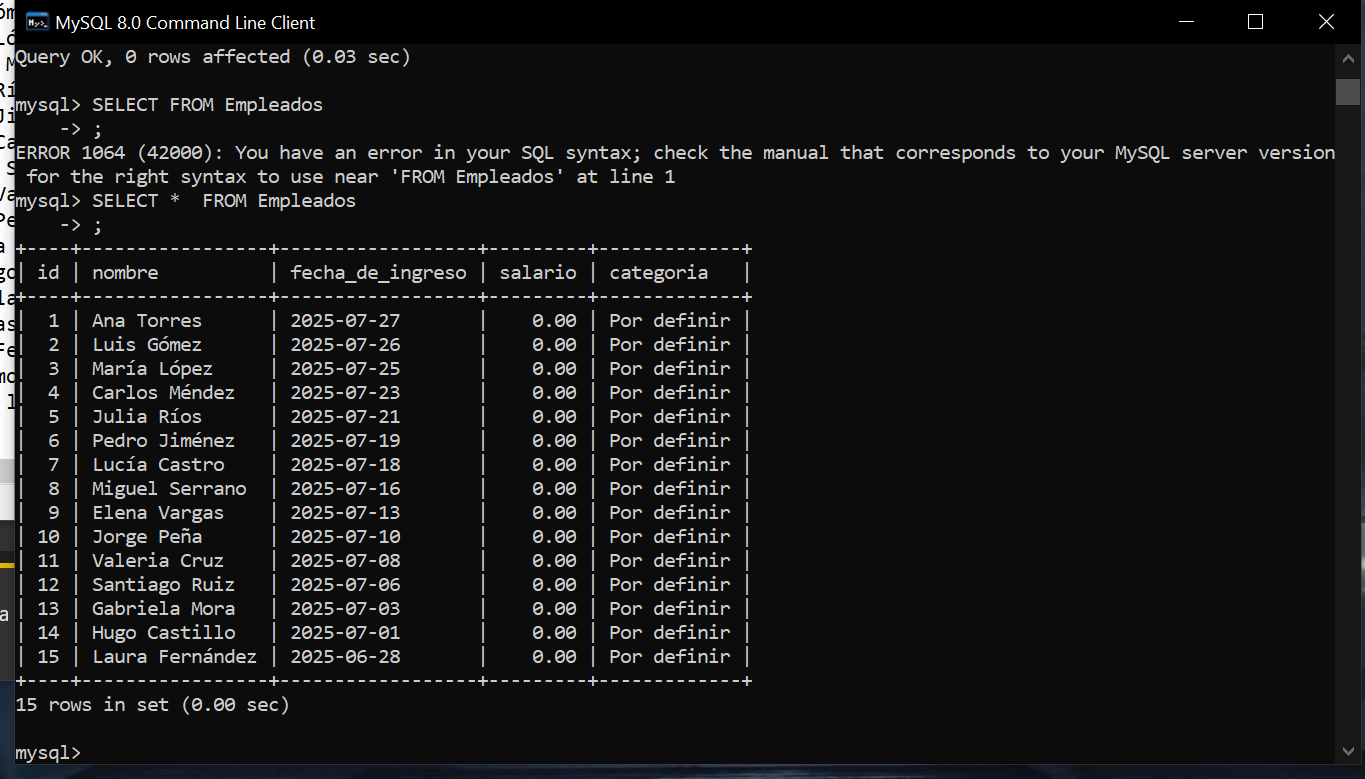
\includegraphics[width=0.85\textwidth]{EmpleadosInicial.png}
\end{center}

\subsection*{Creación del procedimiento almacenado}
\begin{center}
    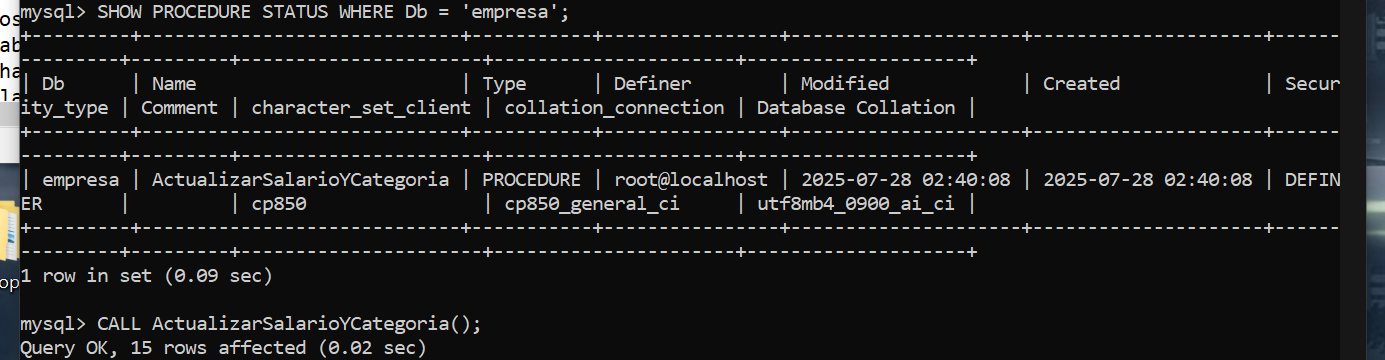
\includegraphics[width=0.85\textwidth]{StoreProcedure.png}
\end{center}

\subsection*{Resultado después de la actualización}
\begin{center}
    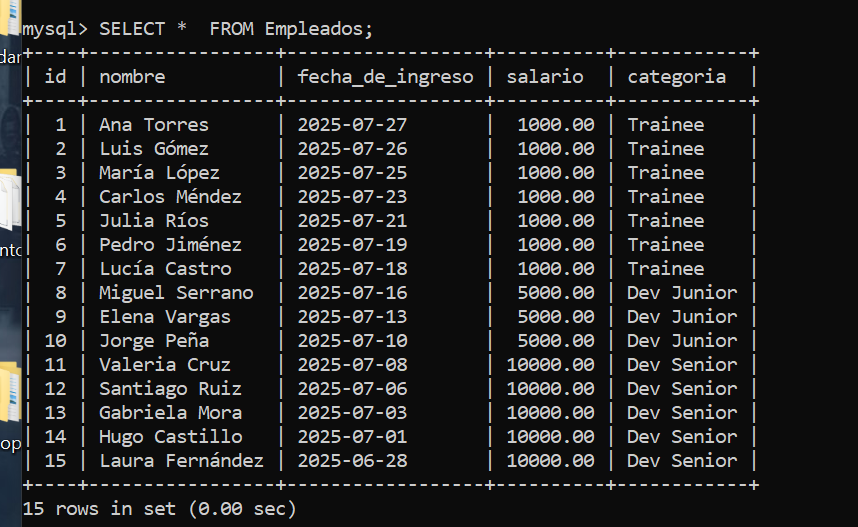
\includegraphics[width=0.85\textwidth]{EmpleadosPrueba.png}
\end{center}

\end{document}
